\chapter[TrabalhosRelacionados]{Trabalhos Relacionados}

\section{sEMG e AM}
Como observado na revisão acadêmica de \cite{yousefi2014characterizing}, os estudos relacionados a sEMG e AM são separados em  dois tipos de transtornos neuromusculares miopatia e neuropatia, onde miopatia refere-se a um grupo de patologias que atingem diretamente o tecido muscular sem relação com disfunções do sistema nervoso. Já a neuropatia, onde encontra-se a doença de Parkinson, é caracterizada por qualquer dano nos nervos envolvidos no controle muscular. Ambos os casos possuem diferenças e similaridades, em resumo segundo \cite{yousefi2014characterizing} as diversas técnicas de AM sobre sEMG, pode-se catalogá-las em três etapas, análise, decomposição e classificação, sendo que não é necessariamente sequencial, podendo ser um processo iterativo.

\subsection{Análise}
O pré-processamento ou análise dos dados é uma das partes mais importantes do processo de aprendizado, essa etapa ocorre apos a coleta dos dados, possuindo alguns objetivos como organizar os dados em conjuntos, identificar possíveis problemas como ruídos ou valores desconhecidos, também é comum utilizar esta etapa para simplesmente aprender mais sobre os modelos plotando gráficos e colhendo mais informações, ou ainda realizar tratamento nos dados como transformações lineares para um conjunto de dados mais simples de ser trabalhado \cite{batista2003pre}. 

\subsection{Decomposição}
Segundo \citeonline{yousefi2014characterizing} a decomposição de um sinal EMG consiste de cinco etapas, aquisição, segmentação, extração de \textit{features}, agrupamento de MUPs e atribuição de MUP.

A seleção das \textit{features} ou características, é a distinção de um sinal bruto em informações úteis, esta informação tratada consiste uma \textit{feature}, a qual será utilizada para treinar o modelo, além disto busca-se remover a parte indesejada do sinal e interferências associadas \cite{phinyomark2012feature}.

Esta etapa deve ser trabalhada cuidadosamente, uma vez que erros podem prejudicar a classificação dos modelos, na pesquisa realizada por \citeonline{phinyomark2012feature} verificou-se que através de gráficos de dispersão, analise estatística e classificação indicou que a maioria das \textit{features} no domínio do tempo são redundantes e desnecessárias, sendo melhor agrupadas em quatro tipos energia e complexidade, frequência, modelo de previsão e dependência do tempo. O estudo recomendou o uso das seguintes \textit{features}:

\begin{itemize}
    \item MAV: método de informação de energia.
    \item WL: informação de complexidade.
    \item WAMP: informação de frequência.
    \item AR: método de predição.
    \item MAVS: depedência  do tempo.
\end{itemize}

Outro estudo que cita algumas \textit{features} compiladas de outros trabalhos, Como observado na figura \ref{featuresEMG}, de acordo com \citeonline{yousefi2014characterizing} as \textit{features} são as seguintes:

\begin{itemize}
    \item \textbf{Amplitude pico a pico}: relaciona os valores nas extremidades minima e máxima de ativação de uma MUP.
    \item \textbf{Tempo de ativação}: descreve a duração entre inicio e termino de ativação de uma MUP.
    \item \textbf{Área de uma MUP}: é obtida integrando á área do sinal gerado, resultante da duração do movimento de uma MUP.
    \item \textbf{Espessura}: é a razão entre a área e a Amplitude.
    \textbf{Tamanho}:
\end{itemize}

\begin{figure}[!htb]
    \centering
     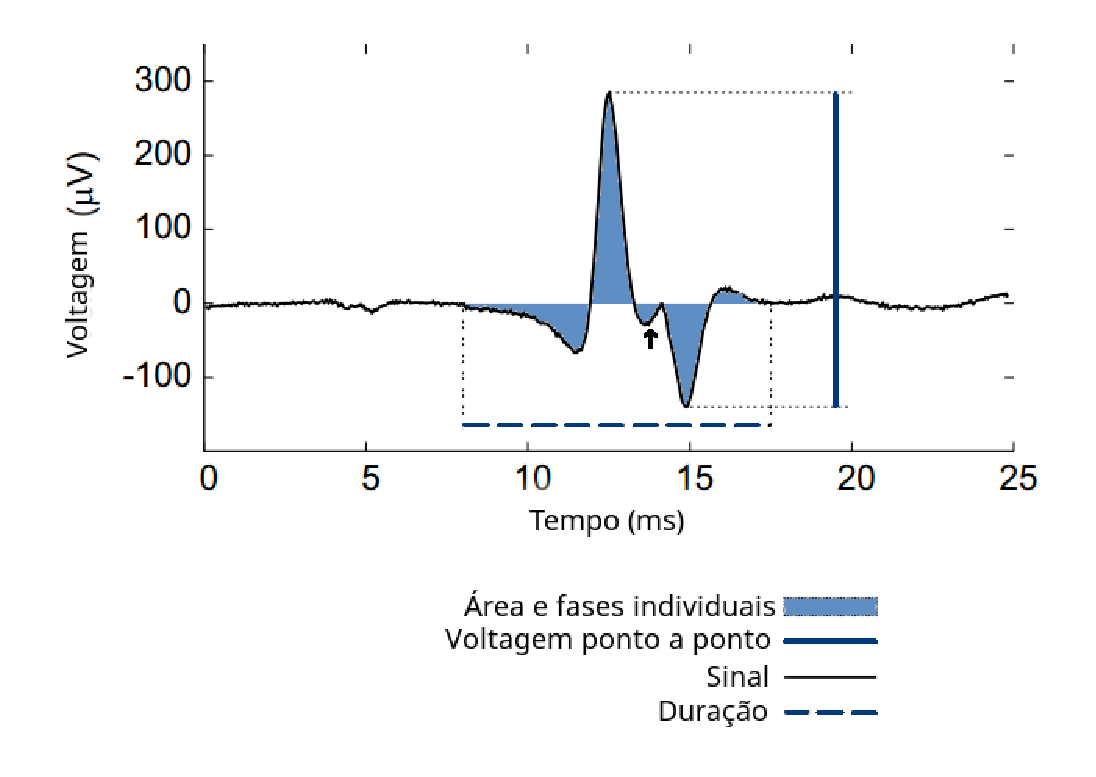
\includegraphics[width=1\textwidth]{figuras/featuresEMG.eps}
     \caption{\textit{Features} de um sinal EMG, adaptado de \citeonline{yousefi2014characterizing}}
     \label{featuresEMG}
 \end{figure}
 

No trabalho realizado por \citeonline{yousefi2014characterizing}, um bom resultado foi obtido na decomposição, onde realizou-se uma classificação utilizando o algorítimo SVM, o qual obteve uma acurácia de 70.4\% no modelo, utilizando uma técnica de extração de \textit{feature} \textit{wavelet}, que utiliza uma função capaz de remodelar uma função no domínio do tempo em diferentes escalas de frequência e tempo, após a utilização desta técnica o algorítimo SVM obteve uma acurácia de 99.3\%.

\section{sEMG, AM e DP}
Existem diversos trabalhos associados a identificação da doença de Parkinson e aprendizado de máquinas, como em \cite{camara2015resting} que utilizou uma rede neural artificial para identificar a doença através do Tremor em repouso, \citeonline{ai2011classification} utilizou sEMG com SVM para identificar a doença de Parkinson e o Tremor essencial, ele utilizou uma a decomposição em modo empírico (do inglês,\textit{empirical mode decomposition} \textbf{EMD} ) para decompor o sinal em funções do modo intrínseco (\textbf{IMF}) e após a decomposição em valores singulares ou \textit{singular value decomposition} (\textbf{SVD}) para extrair as \textit{features} das IMF geradas, e em seguida inseridas no SVM, \citeonline{ai2011classification} também comparou o desempenho substituindo a EMD pela transformada discreta de \textit{wavelets} (\textbf{DWT})  e verificou através de validação cruzada que o método EMD-SVD foi superior ao método DWT-SVD.

SVM também foi utilizada por \cite{kugler2013automated} que combinou sEMG com sinais de acelerômetro para identificar a doença de Parkinson e o Tremor essencial, para validação foi utilizado a validação cruzada.

Outro trabalho interessante foi realizado por \cite{loconsole2018model}, que propôs uma técnica em 3 estágios para diferenciar portadores da DP, usando analise caligráfica com sEMG, e como classificador foi utilizado uma rede neural artificial alinhada com o SVM.

Um comparativo sobre as estratégias de redução de dimensionalidade das \textit{features} em EMG foi realizado por \cite{liu2014feature} obtendo uma média de 95\% de classificação em 12 \textit{features} selecionadas. 
